\documentclass{article}
\usepackage[utf8]{inputenc} %cp1252 pour Windows, utf8 pour Linux
\usepackage[T1]{fontenc}
\usepackage{lmodern}
\usepackage{graphicx}
\usepackage[frenchb]{babel}
\usepackage{hyperref}
\usepackage[table,xcdraw]{xcolor}
\usepackage{float}

\newcommand{\info}{\texttt}


\title{Algorithmique et Structure de Données 2\\
Rapport Projet 1}
\author{Valentin \bsc{Hénique} \and Corentin \bsc{Chédotal}}
\date{13 Mars 2016}

\begin{document}

\maketitle

\section{Introduction}

Dans le cadre de l'Unité d'Enseignement X4I0030 intitulée "Algorithmique et Structure de Données 2" nous avons été amené à produire un premier projet. Celui-ci consiste en la réalisation d'une structure de données abstraite vue en cours : l'Anneau. Le langage de programmation exigé était le C++. Le but du projet était donc d'implémenter l'Anneau mais d'au moins deux façons différentes afin d'observer les différences que cela engendrerait. Les deux implémentations minimales requises étaient par l'utilisation d'une File et d'une Pile, deux structures de données déja implémentées en C++ respectivement par la \info{queue} et la \info{stack}. Ce rapport détaillera comme demandé nos choix derrière les implémentations et fera apparaître les caractéristiques essentielles de chacune d'entre elle afin de faciliter la différenciation des deux méthodes.

\section{Implémentations}

    \subsection{L'Anneau par File (\info{queue)}}
    
    La première façon de réaliser la structure de données abstraite de l'Anneau de façon concrète que nous avons fait est celle employant la File ou \info{queue} en C++ car elle paraissait la plus facile à implémenter.
    
        \subsubsection{Fonctionnement}
        
        Cette méthode vient donc utiliser le principe de la File FIFO (\emph{First In First Out}) comme container des données qui seront entrées par l'Utilisateur dans l'Anneau. Le fonctionnement comme un Anneau, c'est à dire sans notion de queue ou de tête (qui sont pourtant intrinsèques à la File), est rendu possible en ne permettant l'accès qu'à un point ce qui est déja le cas dans la File (la tête de la File) et la rotation de l'Anneau se fait en faisant en fait tourner l'intégralité des données autour du point d'accès à l'élément courant. Ceci va donner l'illusion de l'absence de tête ou de queue car à chaque fois qu'une donnée arrive à la tête et doit "reculer" elle sera immédiatement remise en queue.
        Voici comment les méthodes de l'Anneau ont été implémentées avec la File :
        \label{TabMethodesFile}
        \begin{itemize}
            \item \info{Anneau()} : Le constructeur de Anneau fait simplement appel au constructeur de la File (\info{queue}) afin de construire la file qui servira à stocker les données
            \item \info{\info{\char`\~Anneau()}} : Le destructeur d'Anneau, il est vide car l'Anneau ne fait pas l'objet d'allocations dynamiques nécessitant d'être détruites à la destruction de l'Anneau
            \item \info{estVide()} : Cette méthode vérifiant si un Anneau est vide fait simplement appel à la méthode incluse dans la File qui fait déjà exactement ceci pour la \info{queue}
            \item \info{ajoute()} : Cette méthode permettant l'ajout d'un élément à l'Anneau utilise directement la méthode ajoutant un élément à la queue de la File
            \item \info{supprime()} : De la même façon que \info{ajoute()} ici la méthode supprimant un élément de l'Anneau fait appel à la méthode de la File supprimant l'élément en tête de celle-ci (ce qui s'avère d'ailleurs être l'élément courant de l'Anneau)
            \item \info{courant()} : Justement, cette méthode retournant l'élément courant de l'Anneau utilise simplement la méthode de \info{queue} retournant l'élément en tête de la File
            \item \info{avance()} : Cette méthode fait tourner l'Anneau en faisant tourner les éléments de la queue de la File vers la tête comme indiqué en \ref{SchemaAvanceFile}
            \item \info{recule()} : \`A l'inverse de \info{avance()} cette méthode va faire tourner l'Anneau en déplaçant tous les éléments de celui-ci autant de fois qu'il y a d'éléments - 1 donnant ainsi l'impression que l'Anneau tournait de la tête vers la queue comme montré en \ref{SchemaReculeFile}
        \end{itemize}
        Enfin nous avons décidé de garder le container par défaut pour la \info{queue}, la \info{deque}. En effet celle-ci serait optimale lors d'ajout en fin ou en début de container alors que son homologue la \info{list} serait préférée lors d'ajout au milieu du container ce qui n'est pas notre cas ici.
        
        \subsubsection{Complexité Temporelle}
        
        Ci-après se trouve le tableau des ordres de grandeur des complexités temporelles des diverses méthodes de l'Anneau implémenté à l'aide de la File.
        \begin{table}[H]
        \centering
        \label{ComplexiteFile}
        \begin{tabular}{|l|l|}
        \hline
        \rowcolor[HTML]{C0C0C0} 
        {\color[HTML]{333333} \textbf{Méthodes}} & \textbf{Complexité} \\ \hline
        \info{Anneau()}                                 &  $\Theta(1)$                   \\ \hline
        \info{\char`\~Anneau()}                                &  $\Theta(1)$                   \\ \hline
        \info{estVide()}                                &  $\Theta(1)$                   \\ \hline
        \info{ajoute()}                                 &  $\Theta(1)$                   \\ \hline
        \info{supprime()}                               &  $\Theta(1)$                   \\ \hline
        \info{courant()}                                &  $\Theta(1)$                   \\ \hline
        \info{avance()}                                 &  $\Theta(1)$                   \\ \hline
        \info{recule()}                                 &  $\Theta(n)$                   \\ \hline
        \end{tabular}
        \caption{Complexité Temporelle par File}
        \end{table}
        
        Après il est évident que les ordres de grandeurs des méthodes ne sont finalement que des indicateurs très abstraits et théoriques du fonctionnement d'une implémentation. Ainsi se trouve ci-dessous comme demandé une étude du temps d'exécution de la fonction \info{dedoublonne()} présentée en \ref{dedoublonne} en fonction du nombre de valeurs stockées dans l'Anneau.
        \begin{figure}[H]
            \begin{center}
                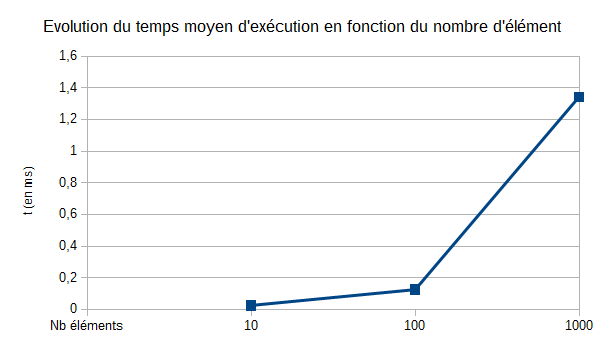
\includegraphics[scale=0.7]{GrapheFile}
                \caption{\label{GrapheFile} Évolution du temps d'exécution par File}
            \end{center}
        \end{figure}
        
        \subsubsection{Encombrement Mémoire}
    
        Enfin l'encombrement mémoire de l'Anneau par File reste relativement limité. En effet le seul attribut de la classe Anneau consiste ici en une seule et unique File (\info{queue}). Or l'empreinte mémoire de celle-ci est plus ou moins proportionnelle au nombre d'éléments de la File, le facteur de proportionnalité dépendant du type de container employé. Ainsi il est tout à fait possible de faire un parallèle avec les complexités temporelles et donner un ordre de grandeur de l'encombrement mémoire de l'Anneau implémenté. Il est donc possible de dire que l'encombrement mémoire est linéaire en fonction du nombre d'éléments dans l'Anneau.
    
    \subsection{L'Anneau par Pile (\info{stack)}}
    
    La deuxième façon d'implémenter de façon concrète la structure de donnée abstraite de l'Anneau que nous avons réalisé est celle employant la structure de Pile ou \info{stack} en C++. Légèrement moins facile à implémenter car le principe même de la Pile force à faire une petite gymnastique mentale afin de garder l'ordre intact lors des déplacement. Enfin comme demandé dans le sujet il est employé non pas une seule mais bien deux Piles dans l'implémentation.
    
        \subsubsection{Fonctionnement}
        
        Cette méthode vient donc employer deux Piles LIFO (\emph{Last In First Out}) comme contenants des données placées par l'Utilisateur dans l'Anneau. En réalité une seule des deux Piles contiendra les données de manière générale mais de part le fonctionnement même de la Pile (l'ajout et suppression ne pouvant se faire qu'en tête) il était essentiel d'avoir une Pile de plus stockant les données de façon à pouvoir les faire "tourner" dans l'Anneau sans changer l'ordre de celles-ci. Le fonctionnement comme un Anneau est justement rendu possible en ayant qu'un seul point d'accès, l'élément courant (qui ici est la tête de la Pile) et la rotation de l'Anneau est rendue possible par une série d'empilement-dépilement de la Pile principale à celle temporaire. Cette série d'opérations est responsable de 'illusion d'une absence de tête et de queue pour l'Utilisateur qui à l'emploi de l'Anneau ne verra que ses données "tournant" par rapport au courant qui est "fixe".\\
        Les méthodes de l'Anneau sont presque toute implémentées de la même façon que par File (\ref{TabMethodesFile}), il ne sera donc détaillé ci après que les méthodes dont l'implémentation diffère vraiment de part l'utilisation de Piles plutôt que d'une File.
        \begin{itemize}
            \item \info{ajoute()} : La méthode permettant d'ajouter un élément dans l'Anneau nécessite ici d'abord d'empiler tous les éléments de l'Anneau dans la Pile temporaire avant d'ajouter le nouvelle élément puis de tout réempiler sur la Pile principale par dessus le nouvel élément; ceci afin de conserver l'ordre des données
            \item \info{avance()} : Cette méthode faisant avancer les données en tournant l'Anneau nécessite à nouveau des dépilement et empilement vers et depuis la Pile temporaire avec le cas particulier de l'élément courant qui doit être mis de la tête de la Pile principale à la base de celle-ci donnant l'impression d'absence de tête et queue. La rotation se fait dans ce cas de la base vers la tête comme montré en \ref{SchemaAvancePile}
            \item \info{recule()} : \`A l'inverse de \info{avance()} le principe reste le même avec dépilement et empilement seulement là c'est la tête de la Pile temporaire soit la base de la Pile standard que l'on essaye de déplacer en tête de la Pile de stockage; ainsi la rotation va se faire de la tête vers la base comme visible en \ref{SchemaReculePile}
        \end{itemize}
        Enfin, suivant le même raisonnement que pour l'implémentation par File nous avons décidé de conserver la \info{deque} comme container des données de la Pile car elle est plus adaptée aux accès aux données que nous faisons que son alternative, la \info{list}.
        
        \subsubsection{Complexité Temporelle}
        
        Ci-dessous se trouve un tableau des ordres de grandeur des complexités temporelles des diverses méthodes de l'Anneau implémentés à l'aide de deux Piles.
        
        \begin{table}[H]
        \centering
        \label{ComplexitePile}
        \begin{tabular}{|l|l|}
        \hline
        \rowcolor[HTML]{C0C0C0} 
        {\color[HTML]{333333} \textbf{Méthodes}} & \textbf{Complexité} \\ \hline
        \info{Anneau()}                                 &  $\Theta(1)$                   \\ \hline
        \info{\char`\~Anneau()}                                &  $\Theta(1)$                   \\ \hline
        \info{estVide()}                                &  $\Theta(1)$                   \\ \hline
        \info{ajoute()}                                 &  $\Theta(n)$                   \\ \hline
        \info{supprime()}                               &  $\Theta(1)$                   \\ \hline
        \info{courant()}                                &  $\Theta(1)$                   \\ \hline
        \info{avance()}                                 &  $\Theta(n)$                   \\ \hline
        \info{recule()}                                 &  $\Theta(n)$                   \\ \hline
        \end{tabular}
        \caption{Complexité Temporelle par Pile}
        \end{table}
        De la même façon que pour la partie précédente sur l'implémentation par File il est évident que les ordres de grandeurs des méthodes ne sont que des représentations abstraites et théoriques du fonctionnement d'un algorithme. Il est toujours très intéressant d'évaluer le fonctionnement d'une implémentation dans un cas concret. Ce faisant vous trouverez ci-dessous, et comme demandé dans le sujet, une étude du temps d'exécution de la fonction \info{dedoublonne()} présentée en \ref{dedoublonne} en fonction du nombre de valeurs stockées dans l'Anneau.
        \begin{figure}[H]
            \begin{center}
                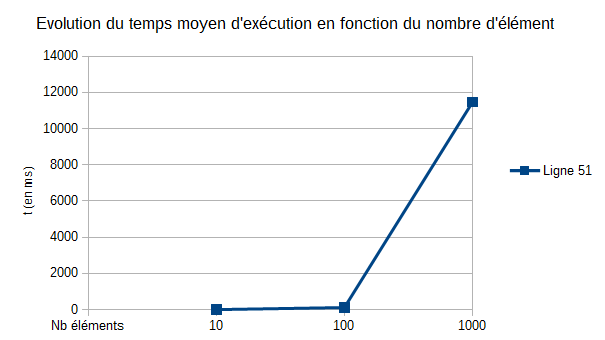
\includegraphics[scale=0.7]{GraphePile}
                \caption{\label{GraphePile} Évolution du temps d'exécution par Pile}
            \end{center}
        \end{figure}
        
        \subsubsection{Encombrement Mémoire}
        
        Enfin de la même manière qu'il est possible de donner des ordres de grandeurs de complexités temporelles il est possible de donner des ordres de grandeur de l'encombrement mémoire d'une implémentation. Or ici les deux seuls attributs sont les deux Piles or l'encombrement mémoire d'une Pile est plus ou moins proportionnel au nombre d'éléments dans celle-ci. Le facteur de proportionnalité dépendant du container de données employé dans la Pile en question. Il se trouve que dans le cas général une seule des deux Piles n'est remplie cependant il n'en reste pas moins possible de s'arrêter là et dire que l'encombrement mémoire est purement et simplement linéaire dans ce cas. En effet lors d'ajout ou de rotation de l'Anneau les données de la Pile principale sont stockées dans la Pile temporaire puis supprimées de la Pile principale et puis vice-versa. Ainsi il y a deux moments pour chacune de ces opérations durant lesquels les deux Piles contiennent l'intégralité des données. L'ordre de grandeur ne change pas vraiment, il s'agit toujours d'une forme linéaire mais il s'agit à ce moment là d'un $2n$ plutôt que d'un $n$. Or si le temps est fondamentalement infini (bien qu'il est évident qu'on ne restera pas devant un programme un siècle durant à attendre un résultat) l'espace mémoire machine ne l'est pas. Il paraissait donc important de noter cette nuance dans le cas d'emploi d'Anneau stockant une très grande quantité de données lourdes.
        
    \subsection{La fonction \info{dedoublonne()}}
    \label{dedoublonne}
    Cette fonction, réalisée comme demandé dans le sujet, sert principalement de banc d'essai des implémentations de la structure de données Anneau. Prenant un Anneau rempli d'éléments en argument elle retournera un Anneau privé des éventuels éléments présents en double ou plus dans la structure retirant donc les doublons d'où son nom. Elle fait cela en déterminant d'abord le compte des éléments à l'intérieur de l'Anneau puis à l'aide de deux boucles imbriquées elle parcourera l'Anneau, pour chaque élément de celui-ci, à la recherche de doublons de l'élément et le cas échéant les supprimera de la structure. Cependant il est très important de noter que pour que \info{dedoublonne()} fonctionne correctement il faut que le type stocké dans l'Anneau donné à la fonction ait un test d'égalité fonctionnel sinon la fonctio peut ne pas agir correctement.
        
\section{Conclusion}

Pour conclure sur ces deux implémentations nous nous rendons très vite compte que l'implémentation par File est bien plus adaptée pour la concrétisation de la structure de données abstraite Anneau que celle employant deux Piles. En effet d'une façon générale la complexité temporelle est bien meilleure par l'utilisation de File que par Piles. En plus de cela l'encombrement mémoire est stable dans le temps quelque soit les opérations faite sur l'Anneau par File alors que certaines opérations sur l'Anneau implémenté par deux Piles voient l'encombrement mémoire doubler pendant un certain temps. Ainsi en plus d'être fixe l'encombrement de la File est égal ou moindre à celui des deux Piles. Enfin et bien que ce ne soit pas une raison à elle seule de choisir l'une ou l'autre méthode il est appréciable de noter que l'implémentation par File en plus d'être la plus efficace était à nos yeux la plus facile à implémenter.

Finalement, pour conclure sur ce projet. Nous sommes plutôt heureux du résultat et ce projet nous a permis aussi de découvrir \emph{Git} nous permettant une bien plus grande aisance de travail à distance. Cela s'est révélé particulièrement important car malgré nos efforts nous avons été poussé par le temps et bien que jamais en retard la date butoir a été à l'origine de quelques stress.

\newpage
\appendix

\section*{Annexe}

\begin{figure}[H]
    \begin{center}
        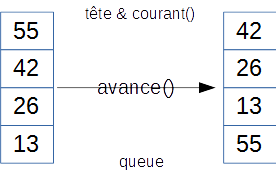
\includegraphics[scale=0.75]{SchemaAvanceFile}
        \caption{\label{SchemaAvanceFile} Évolution d'une File donnée suite à \info{avance()}}
    \end{center}
\end{figure}
\begin{figure}[H]
    \begin{center}
        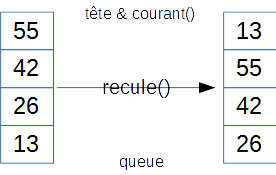
\includegraphics[scale=0.75]{SchemaReculeFile}
        \caption{\label{SchemaReculeFile} Évolution d'une File donnée suite à \info{recule()}}
    \end{center}
\end{figure}
\begin{figure}[H]
    \begin{center}
        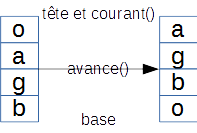
\includegraphics{SchemaAvancePile}
        \caption{\label{SchemaAvancePile} Évolution d'une Pile donnée suite à \info{avance()}}
    \end{center}
\end{figure}
\begin{figure}[H]
    \begin{center}
        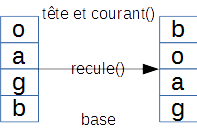
\includegraphics{SchemaReculePile}
        \caption{\label{SchemaReculePile} Évolution d'une Pile donnée suite à \info{recule()}}
    \end{center}
\end{figure}


\newpage
\tableofcontents

\end{document}
